\chapter{Maiden Voyage}

After the boat had arrived and was properly equipped, everything was ready for a basic test with simple, manual control in order to observe its stability, its ability to take turns, as well as the speed the ship could navigate at. Because all pools or other forms of standing water were frozen at the time, this test had to be performed at the marina located \href{https://maps.google.com/?ll=57.058301,9.896772&spn=0.003495,0.009645&t=h&z=17""}{here}, on the corner of Skudehanvnsvej and Vestre Fjordvej, 

In picture \vref{fig:GpsOnMap}, the data obtained from the GPS sensor during this trip is plotted on top of an Open Street map of the harbor in which it took place. 

Both Figure \vref{fig:ship_turning2} and \vref{fig:ship_turning} represent the ship in a continuous spiral. The turning radius will depend on the difference between the two motor speeds. It can be seen from the figures that this radius can be as small as 1 meter, which is a very good response.

\begin{figure}[htbp]
	\begin{center}
		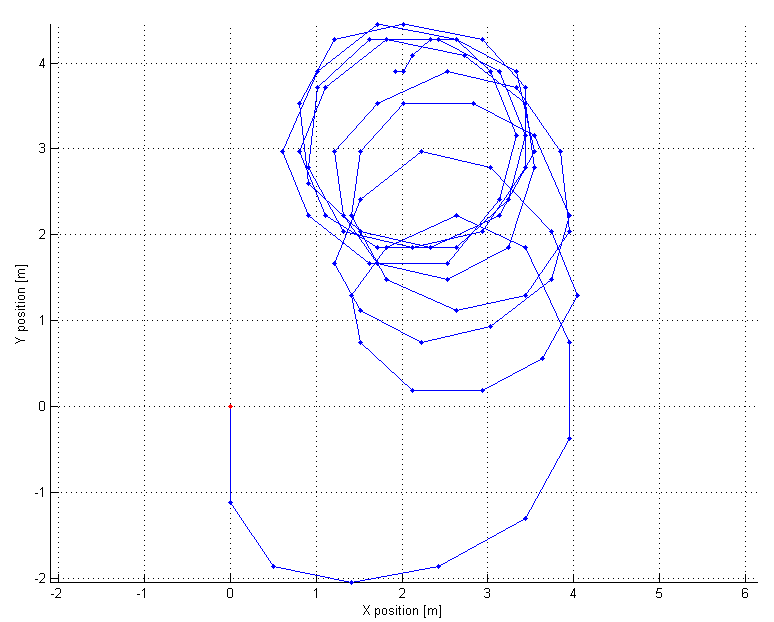
\includegraphics[width=\textwidth]{img/maidenVoyage/ship_turning2}     
		\caption{GPS measurements of ship turning as logged by the LLI during maiden voyage} 
		\label{fig:ship_turning2}               
	\end{center}   
\end{figure}

\begin{figure}[htbp]
	\begin{center}
		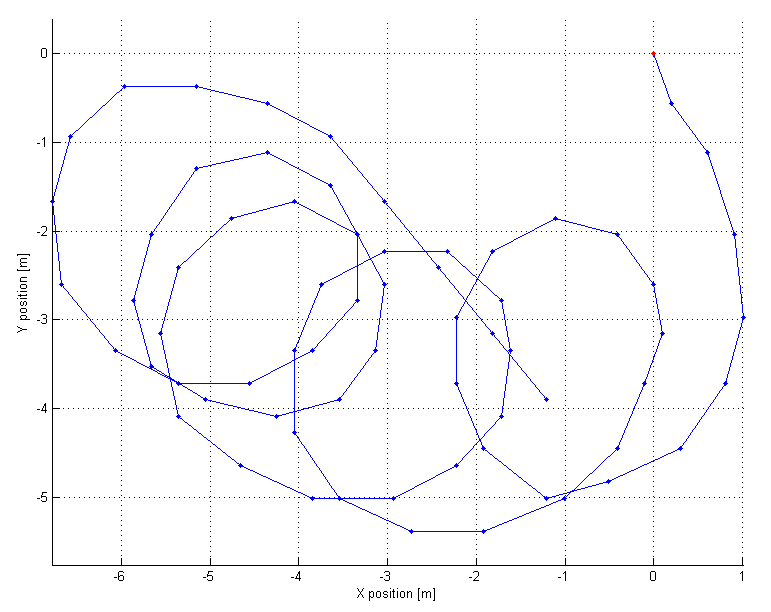
\includegraphics[width=\textwidth]{img/maidenVoyage/ship_turning}     
		\caption{GPS measurements of ship turning as logged by the LLI during maiden voyage} 
		\label{fig:ship_turning}               
	\end{center}   
\end{figure}

